\pdfoutput=1

\documentclass{l4proj}

\usepackage{hyperref}
\hypersetup{
  colorlinks=false,
    citebordercolor={0 1 0},
    filebordercolor={1 1 0},
    linkbordercolor={1 0 0},
    urlbordercolor={0 1 1}
}
\usepackage{caption}
%\usepackage[all]{hypcap}
\usepackage{listings}

\usepackage{chngcntr}
\counterwithout{figure}{chapter}
\counterwithout{table}{chapter}
\AtBeginDocument{\counterwithout{lstlisting}{chapter}}

\lstset{ %
basicstyle=\scriptsize\ttfamily,     % the size of the fonts that are used for the code
%basicstyle=\tiny,     % the size of the fonts that are used for the code
numbers=left,               % where to put the line-numbers
%numberstyle=\tiny,    % the size of the fonts that are used for the line-numbers
numberstyle=\scriptsize,    % the size of the fonts that are used for the line-numbers
numbersep=10pt,             % how far the line-numbers are from the code
frame=trBL,                 % adds a frame around the code
%tabsize=2,                  % sets default tabsize to 2 spaces
captionpos=b,               % sets the caption-position to bottom
breaklines=true,            % sets automatic line breaking
breakatwhitespace=false,    % sets if automatic breaks should only happen at whitespace
showstringspaces=false,     % Don't show underscores as space characters
frameround=fttt
}

\begin{document}
\title{Exploring the possibility of accelerating Hurricane Simulator \\ using Apache Spark framework}
\author{Andrej Hoos}
%\date{March ???, 2016}
\maketitle

\begin{abstract}
Large Eddy Simulator is a high resolution meteorological simulator designed to model
flows over urban topologies. While the simulation has been accelerated with the use of 
OpenCL technology, there are still limits to the size of the simulation that can be run on a single computer.

This project tries to overcome this limitation by parallelising the simulation on a 
network cluster using Apache Spark framework. Suitability of multiple approaches to 
halo exchanges over network is explored and it is demonstrated that such exchange 
can be done using MapReduce frameworks and Apache Spark specifically. The simulation 
is rewritten from Fortran to Java and uses Aparapi for OpenCL acceleration and Java Native Access 
to access Fortran routines in the original code. A number of simple test was conducted 
to determine the scalability and viability of this method. However, significantly 
decreased performance was observed when compared to the non-parallelised implementation 
due to framework overhead.
\end{abstract}

\educationalconsent
%
%NOTE: if you include the educationalconsent (above) and your project is graded an A then
%      it may be entered in the CS Hall of Fame
%

\newpage
\vspace*{\fill}
\section*{\centering Acknowledgments}
First, I would like to thank my supervisor, Dr Vanderbauwhede for proposing an interesting
project and for providing interesting pieces of information during our meetings.

I would also like to thank Oren Segal for answering my questions and providing hints about 
Apache Spark and Aparapi, as well for prividing the aparapi-ucores library.
\vspace*{\fill}

\tableofcontents
%==============================================================================

%==============================================================================
%  Introduction
%==============================================================================
\chapter{Introduction}
\pagenumbering{arabic}

Simulating real world weather system is a difficult task, requiring a lot of computational power.
One such simulator is The Large Eddy Simulator for the Study of Urban Boundary-layer Flows (LES)
developed by  Hiromasa Nakayama and Haruyasu Nagai at the Japan Atomic Energy Agency
and Prof. Tetsuya Takemi at the Disaster Prevention Research Institute of Kyoto University~\cite{les_analysis}~\cite{les}.
It simulates meteorological systems in an urban environment with building resolution.
Originally, LES is implemented in Fortran 77 with no explicit parallelization.

\section{Motivation \& Aim}

As multi core computational devices are now commonplace, parallelisation has become
a important consideration when implementing simulations. Therefore LES has been
ported to Fortran 95/OpenCL implementation by Wim Vanderbauwhed~\cite{les_wim}. Using this implementation,
LES can be run parallelised on any OpenCL compatible computational device, which shows
significant improvements in speed. While these improvements can be used to reduce the time needed to
run single simulation run or to increase the size of the spatial domain of the simulation,
there are limits to both. One of these limits is number of computational units the device has,
limiting the extent of parallelization. The other is memory available on the device.

Using a network cluster of computers can, in theory, help overcome these limits to some extent.
However, splitting work onto multiple nodes in a cluster introduces a issue of communicating
important information over network. Specifically, in case of LES, data that is at the boundary of
the spatial domain of each node needs to be exchanged in so called halo exchanges.

Recently, there has been a rise in a new computational frameworks focused on working in
distributed environment. One of these frameworks is Apache Spark which is based on
the MapReduce parallel execution paradigm.

The aim of this report is to explore the possibility of using the Apache Spark in Java to parallelise
LES, or any algorithm relying on halo exchanges in network distributed environment.

\section{Outline}

Further background will be described in \autoref{chap:background}, including information
on LES, Apache Spark, OpenCL and related work. Implementation of halo exchanges in 
Apache Spark will be discussed in \autoref{chap:halos} and \autoref{chap:les_java} will
explain the process of porting LES code from Fortran to Java. Evaluation of the achieved
performance can be found in \autoref{chap:eval} and \autoref{chap:conclusion} contains
final remarks and notes about future work.

%==============================================================================
%  Background
%==============================================================================
\chapter{Background}
\label{chap:background}

\section{Large Eddy Simulator}

The Large Eddy Simulator for the Study of Urban Boundary-layer Flows developed by
Disaster Prevention Research Institute of Kyoto University is a high resolution
meteorological simulator designed to model turbulent flows over urban topologies. 
It achieves this by using mesoscale meteorological simulations and building resolving
large-eddy simulations. It also uses The Weather Research and Forecasting Model~\footnote{\url{http://www.wrf-model.org}}
to compute the wind profile as an input for the simulation. The simulation is split into
multiple subroutines, however, the most important one is the Poisson Equation solver.
This is the most computationally intensive subroutine and it uses successive over relaxation to solve
a linear system of equations. Each time step of the simulation needs to execute following subroutines
in a sequence:

\begin{tabular}{ | l | l | }
  \hline  
  \textbf{velnw} & Update velocity for current time step \\
  \textbf{bondv1} & Calculate boundary conditions (initial wind profile, inflow, outflow) \\
  \textbf{velfg} & Calculate the body force \\
  \textbf{feedbf} & Calculation of building effects \\
  \textbf{les} & Calculation of viscosity terms (Smagorinsky model) \\
  \textbf{adam} & Adams-Bashforth time integration \\
  \textbf{press} & Solving of Poisson equation (SOR) \\
  \hline  
\end{tabular}

The simulator was originally written in Fortran 77. The current version was ported to Fortran 95
and accelerated using OpenCL in work by Wim Vanderbauwhed~\cite{les_wim}.

LES runs over spatial domain represent by a 3D grid. Size of 150x150x90 is used for the most
of this report, but the size can be varied in x and y direction. By increasing the size of the
grid in x and y directions, LES can be run with higher resolution, or it can used 
to cover larger area. However doing this increases the time needed to complete the simulation
and more importantly there is a limit to how big the grid can be so that it fits inside the RAM.

\subsection{Parallelisation}

Using a cluster of computers, we can split the domain such that every node in the cluster runs
LES on a small portion of the domain. This allows to run LES on much larger domain than what would be
possible on a single computer. To run LES correctly in this scenario, each node needs access to the 
boundary data belonging to each of its eight neighbours (figure~\ref{fig:neighbours}).

\begin{figure}
\centering
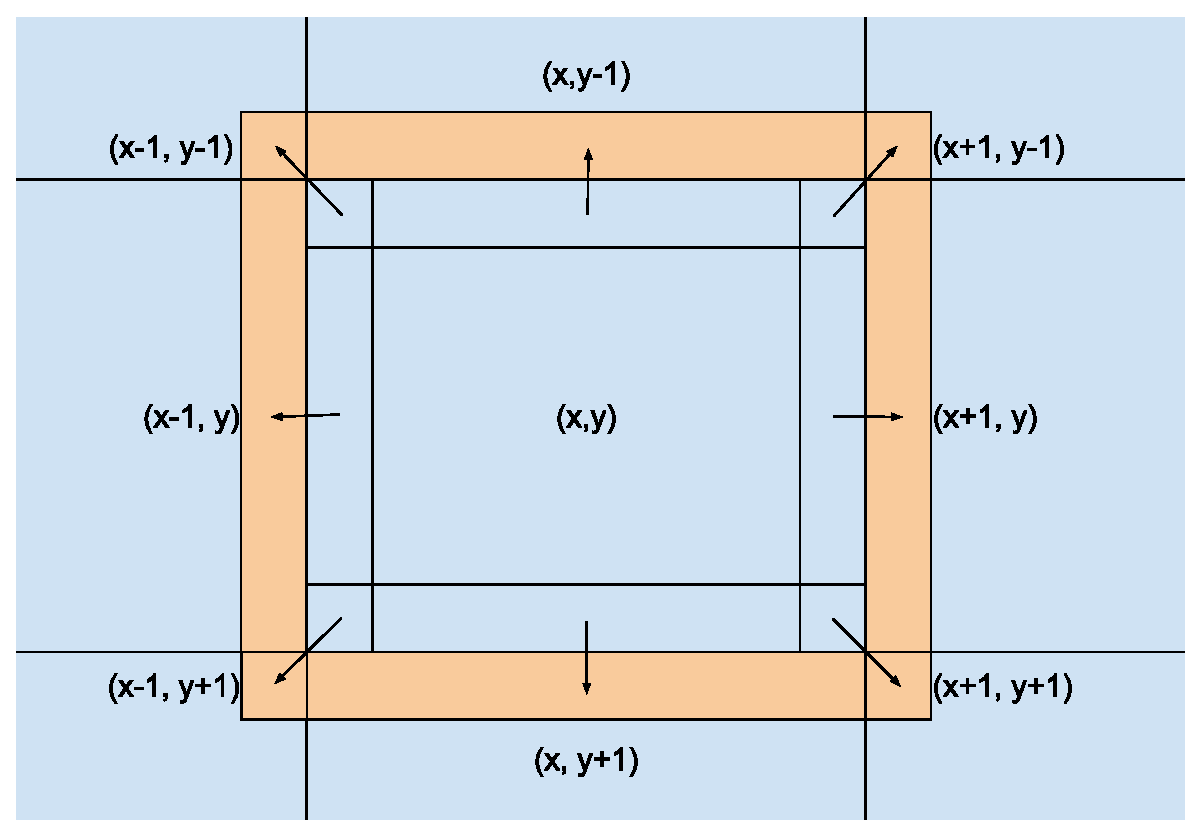
\includegraphics[width=0.7\textwidth]{images/Neighbour_exchange.eps}
\caption{Node (x,y) needs access to the edges of all its neighbours}
\label{fig:neighbours}
\end{figure}

Message Passing Interface (MPI)
~\footnote{\url{http://www.mcs.anl.gov/research/projects/mpi/mpi-standard/mpi-report-2.0/mpi2-report.htm}} 
is considered to be most commonly used for communication in distributed memory environments.
Because of this, LES has already been parallelised using MPI by Gordon Reid as his MSci project at University of Glasgow~\cite{les_mpi} and others~\cite{les_palm}. Although MPI is considered standard and achieves good performance, it
is not an easy task to parallelise algorithms using MPI, especially for scientists with minimal
experience with Computing Science. Therefore, it is important to investigate the possibilty
of using frameworks with higher level abstraction and that are easy to deploy on a standard
network cluster.

\section{MapReduce parallel processing}

MapReduce is a programming model used mainly for processing large quantities of data
and is intended to be used on network clusters~\cite{map_reduce}. Programs using this model consist of Map and Reduces
methods which are automatically parallelised. MapReduce was originally the name of a technology by
Google, but is now used for the model in general. MapReduce libraries and frameworks are now 
available in many programming languages.

MapReduce model usually operates on key-value pairs and can be described by three main steps:

\begin{itemize}  
\item \textbf{Map}: \textbf{map()} function is applied to all of the pairs, creating a collection of new key-value pairs
\item \textbf{Shuffle}: the output data is redistributed across network such that pairs with the same key are located on the same node
\item \textbf{Reduce}: the output data is processed by applying the \textbf{reduce()} function to the output pairs
\end{itemize}

Advantage of using MapReduce is that only map() and reduce() functions need to be written and
the shuffle step is handled automatically by the library or framework and is usually optimised. 
In addition, most MapReduce frameworks provided more data manipulation methods such as grouping or 
joining.

\subsection{Apache Spark}

Apache Spark~\footnote{\url{http://spark.apache.org/}} is one of these frameworks and is 
available in Java, Scala, Python and R. It claims to be faster over alternatives such as 
Apache Hadoop, because it allows MapReduce to run in memory as opposed to reading and 
writing inputs and outputs solely from disk. This, with combination of its increasing 
community and high-level abstraction makes this framework suitable for the purposes of this project.  

Every Spark program consists of a driver program and a worker node(s). When Spark is
used in cluster mode, a cluster manager is also required (figure~\ref{fig:spark}). Cluster manager allocates resources
across nodes and is usually referred to as Spark master in this report. Once the driver 
program connects to the cluster, it acquires executors on the worker nodes and
starts sending tasks for them to execute.

The driver program runs the user's main function and allows to run parallel operations on the cluster.
The main abstraction provided by spark is represented by resilient distributed dataset (RDD). RDD is
a collection of elements which is automatically distributed across the cluster that can be operated on
in parallel.

Listing~\ref{lst:spark} shows an example Spark program which loads a text file and creates a RDD
containing words from the file. It then uses \texttt{mapToPair} to create key value pairs, where 
key is a word a value is count and then produces counts of each word by using \texttt{reduceByKey}.

\begin{figure}
\centering
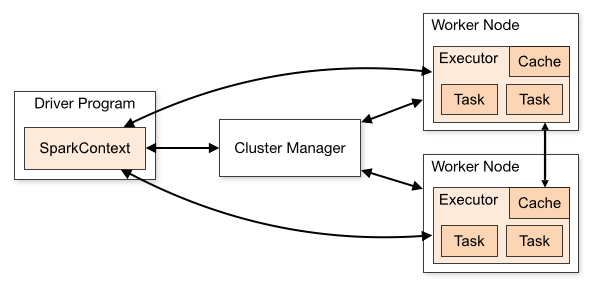
\includegraphics[width=0.7\textwidth]{images/spark.png}
\caption{Apache Spark cluster components overview ~\protect\footnotemark}
\label{fig:spark}
\end{figure}
\footnotetext{\url{http://spark.apache.org/docs/1.4.1/cluster-overview.html}}

\begin{figure}
  \lstset{caption={Example Spark program},label={lst:spark}}
  \begin{lstlisting}[language=Java]
SparkConf conf = new SparkConf().setAppName(appName).setMaster(master);
JavaSparkContext sc = new JavaSparkContext(conf);

JavaRDD<String> textFile = sc.textFile("...");
JavaRDD<String> words = textFile.flatMap(new FlatMapFunction<String, String>() {
  public Iterable<String> call(String s) { return Arrays.asList(s.split(" ")); }
});
JavaPairRDD<String, Integer> pairs = words.mapToPair(new PairFunction<String, String, Integer>() {
  public Tuple2<String, Integer> call(String s) { return new Tuple2<String, Integer>(s, 1); }
});
JavaPairRDD<String, Integer> counts = pairs.reduceByKey(new Function2<Integer, Integer, Integer>() {
  public Integer call(Integer a, Integer b) { return a + b; }
});
counts.saveAsTextFile("...");
  \end{lstlisting}
\end{figure}

\section{OpenCL}

OpenCL~\footnote{\url{https://www.khronos.org/opencl/}} is a framework that allows
writing parallelised software on various computational platforms, such as CPUs, 
GPUs and hardware accelerators. OpenCL uses own programming language based on C99 for 
executing programs called kernels. These kernels can be run across multiple devices 
with almost no modification. The differences in code are usually caused by different 
feature sets on different devices (e.g. double floating point precision support), or by
different performance of specific operations.

\subsection{Structure overview}

OpenCL architecture consists of a host and a computational device connected to the host.
The host is usually the CPU and it handles the initialisation, allocating memory, queuing work
and harvesting of results from the computational device. The computation device usually has one
or more compute units and each compute unit consists of multiple processing elements. A single kernel
execution usually runs on multiple processing elements in parallel.

A work item is the smallest control flow unit in the OpenCL architecture. A work group is a 
collection of related work items, which execute the same kernel and share local memory.
The size of the work group is limited by the underlying device and can usually consist of up to 
three dimensions.

\begin{figure}
\centering
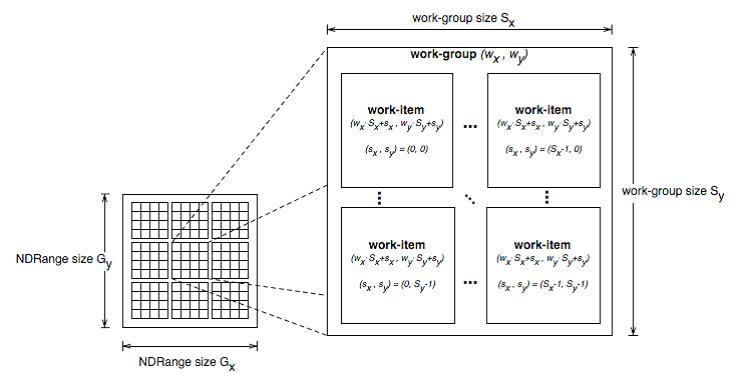
\includegraphics[width=0.8\textwidth]{images/opencl.jpg}
\caption{Work structure in OpenCL ~\protect\footnotemark}
\label{fig:opencl}
\end{figure}
\footnotetext{\url{https://software.intel.com/sites/landingpage/opencl/optimization-guide/Basic_Concepts.htm}}

When executing the kernel, the host code specifies the global work size. The host can specify 
the size of the work groups the work is divided into, or it can be left to implementation do be decided
automatically. The kernel is then executed on each work item, which can determine its portion 
of work by accessing its global or local id. The figure~\ref{fig:opencl} shows the overall work structure in OpenCL.

\subsection{Kernels}

Kernels are OpenCL programs executed in parallel on a computation device. The language that is
used to write kernels is based on C99, but adapted to fit the OpenCL device model. It replaces 
the C standard version library with custom set of functions, which contains additional features, such as 
math functions. When using pointers, programmer can use region qualifiers annotations, such as
\texttt{\_\_global} or \texttt{\_\_local}, which specify a level in memory hierarchy. Besides standard
types like \texttt{float} or \texttt{int}, OpenCL defines vector types with fixed length
of 2, 4, 8 or 16. Operations on these vector types are intended to map onto vector instructions on the device.
The entry point functions are marked with \texttt{\_\_kernel} which signals that it can be called by the host code.

The host code is responsible for selecting the device, loading the kernel code and building the 
program using the selected device. The program can be than queued, which also involves specifying
the global work size, and optionally the local work size.

\subsection{Aparapi}

Aparapi~\footnote{\url{https://aparapi.github.io/}} is an API that allows programmers
to write OpenCL capable parallel programs in Java. Aparapi was originally an AMD 
product~\footnote{\url{http://developer.amd.com/tools-and-sdks/opencl-zone/aparapi/}},
but was released to open source in 2011. It is capable of converting Java bytecode
into OpenCL programs that can be executed on computational devices. Aparapi also 
provides abstraction for selecting devices and queuing programs. 

Listing~\ref{lst:aparapi} shows an example Aparapi program. The example creates two 
vectors, \texttt{a} and \texttt{b} and sums them into vector \texttt{sum}. \texttt{a} and \texttt{b}
are represented by two arrays, which are initialised with random values. The OpenCL program
is created by using a \texttt{Kernel} class with overloaded \texttt{run} method and 
can be enqueued and run using \texttt{execute} method. The underlying OpenCL code that
is used to create the OpenCL program can be seen in listing~\ref{lst:aparapi_cl}.
\begin{figure}
  \lstset{caption={Example Aparapi program that sums two vectors},label={lst:aparapi}}
  \begin{lstlisting}[language=Java]
import com.amd.aparapi.Kernel;
import com.amd.aparapi.Range;

public class VectorAdd 
{
    public static void main( String[] args )
    {
        final int size = 50000000;

        final float[] a = new float[size];
        final float[] b = new float[size];

        for (int i = 0; i < size; i++) {
           a[i] = (float) (Math.random() * 100);
           b[i] = (float) (Math.random() * 100);
        }

        final float[] sum = new float[size];

        Kernel kernel = new Kernel(){
           @Override public void run() {
              int gid = getGlobalId();
              sum[gid] = a[gid] + b[gid];
           }
        };
        
        kernel.execute(Range.create(size));
    }
}    
  \end{lstlisting}
\end{figure}

\begin{figure}
  \lstset{caption={OpenCL code generated by the Aparapi example},label={lst:aparapi_cl}}
  \begin{lstlisting}[language=C]
typedef struct This_s{
   __global float *val$sum;
   __global float *val$a;
   __global float *val$b;
   int passid;
}This;
int get_pass_id(This *this){
   return this->passid;
}
__kernel void run(
   __global float *val$sum, 
   __global float *val$a, 
   __global float *val$b, 
   int passid
){
   This thisStruct;
   This* this=&thisStruct;
   this->val$sum = val$sum;
   this->val$a = val$a;
   this->val$b = val$b;
   this->passid = passid;
   {
      int gid = get_global_id(0);
      this->val$sum[gid]  = this->val$a[gid] + this->val$b[gid];
      return;
   }
}   
  \end{lstlisting}
\end{figure}

\section{Related work}

Parallelised version of LES has been created by Gordon Reid~\cite{les_mpi} using MPI
and Glasgow Model Coupling Framework (GMFC). The work creates MPI implementation for both shared-
and distributed-memory systems. GMFC implementation is created for shared-memory systems.
The implementation is evaluated using constant global area as well as using expanding area
test with each node having area of the same size. Both MPI and GMCF have been shown
to scale well using both evaluation methods.

Another work to Parellise LES is work by Raasch and Schröter \cite{les_palm}. The work
uses different LES implementation from the one used in this project. Parallelisation
using MPI is shown to speed up the simulation on both small domain and large domains.

Using Apache Spark for halo exchanges seems to be not well researched use case, although
one work~\cite{seismic_spark} has used Spark to solve a stencil problem computation. 
The work implements Jacobi Stencil Codes algorithm which requires exchange of boundary
data. Three different methods are evaluated. Method using broadcast variables, method
that shares the boundary data using CassandraDB and method that uses boundary RDDs.
Method with broadcast variables is shown to scale well up to around 100 nodes, while
the other methods can scale up to 500 nodes, with the boundary RDDs approach providing
better performance. Unfortunately the work does not describe in detail the implementation
details of this approach.

%==============================================================================
%  Halo exchanges in Spark
%==============================================================================
\chapter{Halo exchanges in Spark}
\label{chap:halos}

The main challenge of this project is to construct viable halo exchange algorithm, using 
data manipulation methods provided by Apache Spark. Multiple possible algorithms were 
considered and their implementation details, advantages and drawbacks are discussed in this chapter.

\section{Game of Life as a proof of concept}
To test the considered algorithms, a implementation of Conway's Game of Life was used.
This was because of its simplicity and becasue it resembles the simulator in that
in needs boundary data to be transfered in order to be parallelised in 
distributed environment.

The Game of Life is a cellular automaton and is run on a 2D grid of cells. To compute
the transition of a single cell, state of each of its eight neighbours are needed.
The transitions are defined as:

\begin{itemize} 
\item Any live cell with fewer than two live neighbours dies.
\item Any live cell with two or three live neighbours lives on to the next generation.
\item Any live cell with more than three live neighbours dies.
\item Any dead cell with exactly three live neighbours becomes a live cell.
\end{itemize}

We can group the cells into same size rectangle shaped chunks and compute the transitions of each
chunk on a separate node of the cluster. The nearest edges of neighbouring
chunks need to be exchanged before each transition in order for the edge cells to know
the state of all of their neighbours. This is the similar case as in LES and is therefore
suitable as a proof of concept.

\section{Broadcast variables}
\label{chap:broadcast}

The simplest way to exchange halos is using broadcast variables. Spark allows to
create a broadcast variable in the driver program, which can be then shipped to worker
nodes if needed. However the limitation is that only the driver program can create
broadcast variables (i.e. they cannot be created in the worker code) and therefore
the workers would need to send their edge data to the driver program, which would
contruct the appropriate halos and create a broadcast variable(figure~\ref{fig:broadcast}).

\begin{figure}
\centering
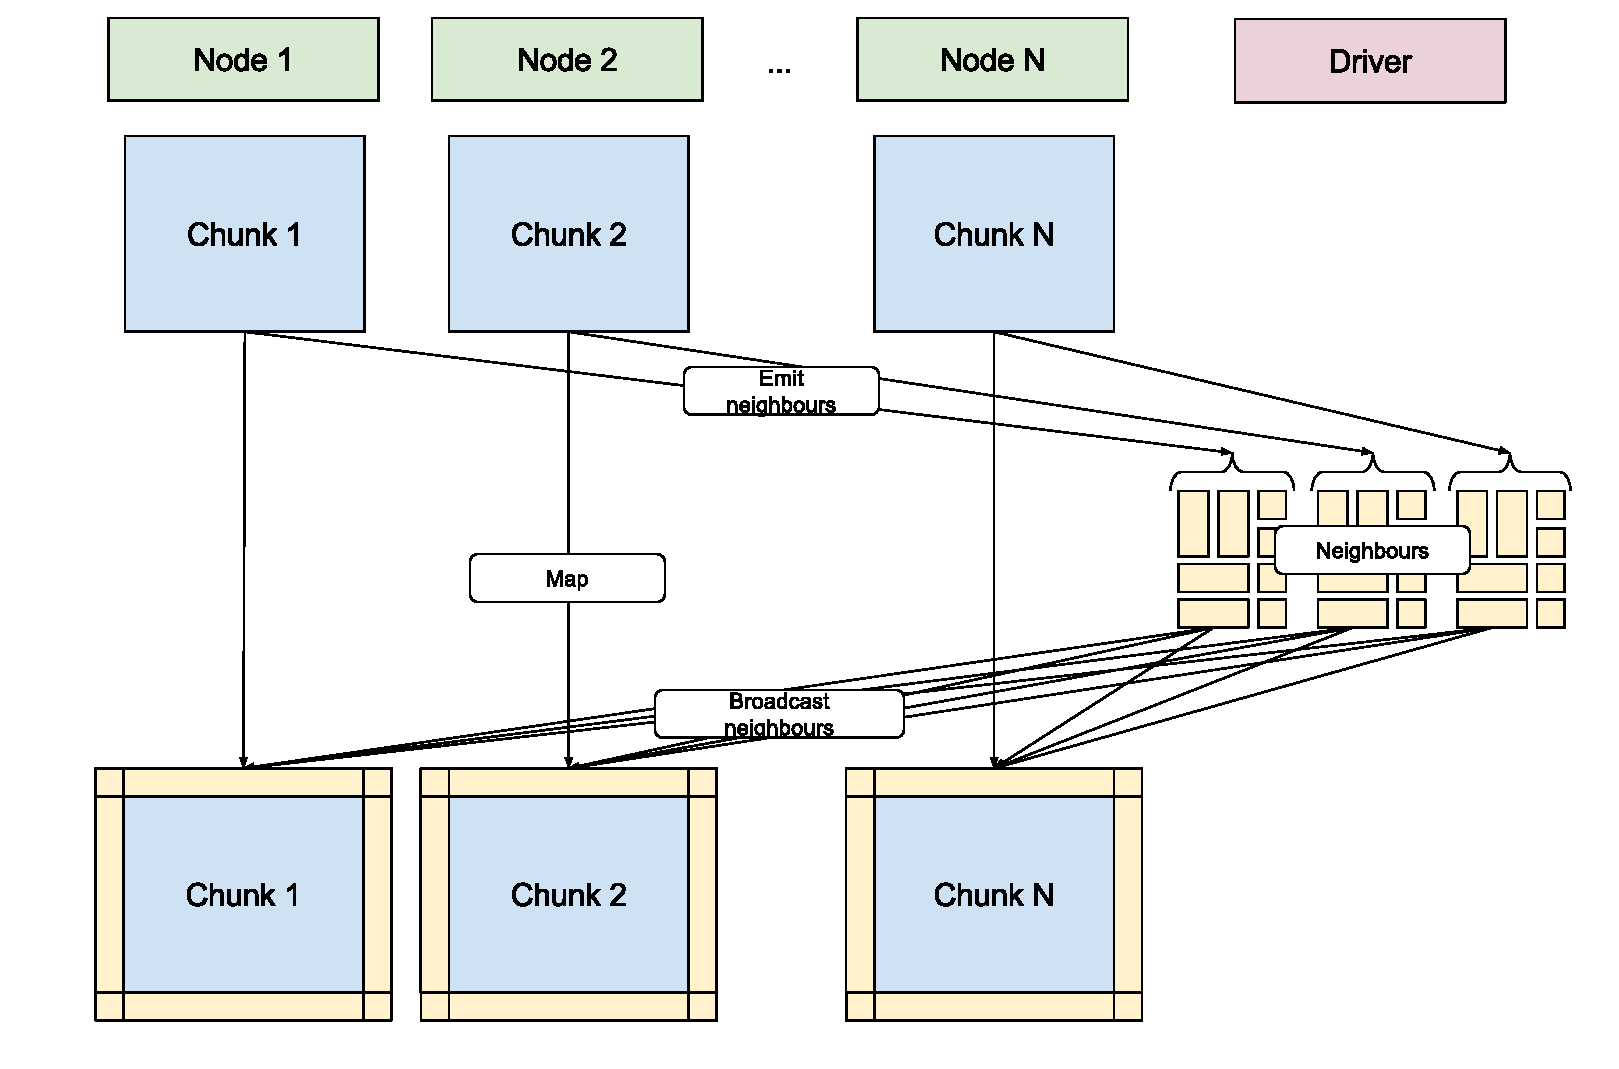
\includegraphics[width=0.9\textwidth]{images/Broadcast_variable.eps}
\caption{Diagram of the the algorithm using broadcast variables}
\label{fig:broadcast}
\end{figure}

This means that the halos would be transferred to their destination always via
the node which hosts the driver program, and therefore the algorithm would do 
twice as much network transfers as the ideal case where the halos are transferred
to their destination directly. Therefore this approach was deemed unsuitable. 

\section{MapReduceByKey}

Another way is to use a combination of map and reduce steps (figure~\ref{fig:map_reduce}). To represent the 
chunks, we use Spark Pair Collection of key-value pairs of key and chunk (\texttt{JavaPairRDD<String, Chunk>}).
The key represents the coordinates of the chunk.

\begin{figure}
\centering
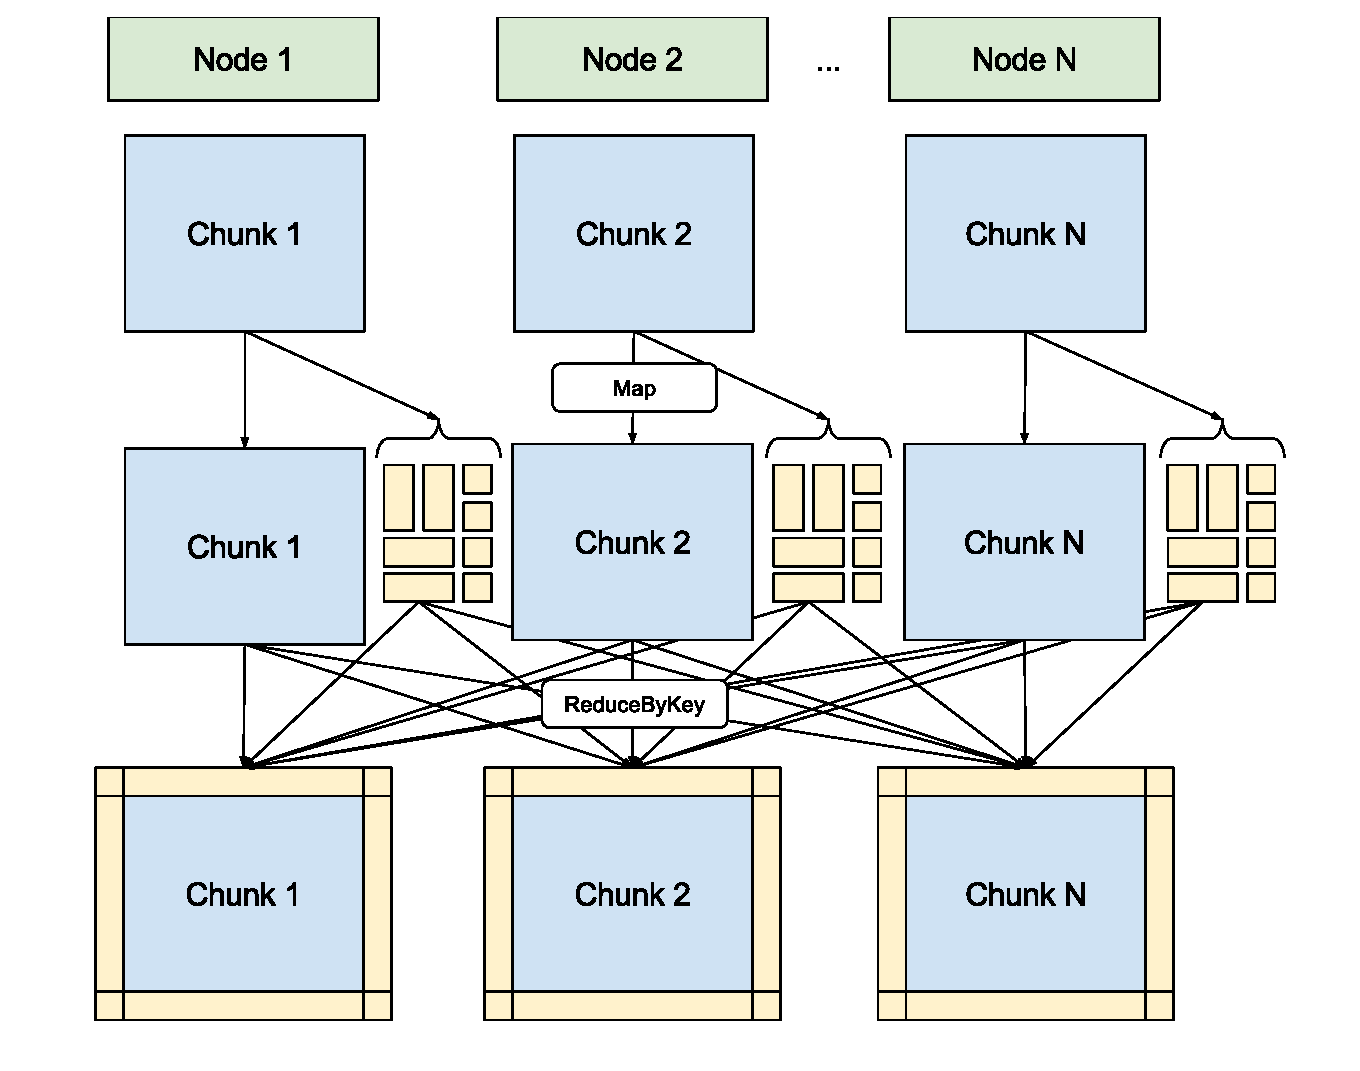
\includegraphics[width=0.9\textwidth]{images/MapReduce.eps}
\caption{Diagram of the the MapReduceByKey algorithm}
\label{fig:map_reduce}
\end{figure}

In the first stage we transform this collection into another collection which contains
the chunks from the original collection together with all neighbours using map
(\texttt{flatMapToPair}). The keys of the neighbours key value pairs are the keys of their respective
target chunk.

The second step then does reduce on this new collection using \texttt{reduceByKey}. 
The reducer function takes a chunk and a neighbour and reduces them into a chunk
with the neighbour added to it, which results in a collection of chunks which are
larger by one cell on each side.

The last step is a map step, which computes next transition on each chunk, returning
collection of transformed chunks which are the original size.

There are, however, some drawbacks to this approach. The first is, that we cannot
control the exact order in which these operations are executed. For example, Spark
might decide to execute the first map step on first two chunks (assuming there are more than two)
and run the reduce step on the results. Then, the first map step might be run on the rest
of the chunks. The second issue is that we cannot control, on which node is each step 
executed. This two issues result in all of the chunks and not only neighbours are
transferred over network, which is unacceptable for the purposes of this project.

\section{MapGroupByKey}

To resolve one of the issues mentioned above, it is possible to replace the reduce
step with group step (figure~\ref{fig:map_group}). This uses \texttt{groupByKey} to group chunk together with
neighbours that share the same key. The grouping function takes the chunk with
its neighbours and combines them into a single chunk, such that the result is the
same as after the reduce step in previous section.

Using this method the issue of the order of execution is solved, since the group
can be executed only after all of first map stage has been executed. The second issue
of not being able to control where each stage is executed still remains and therefore
the issue of transferring all chunk over network remains as well.

\begin{figure}
\centering
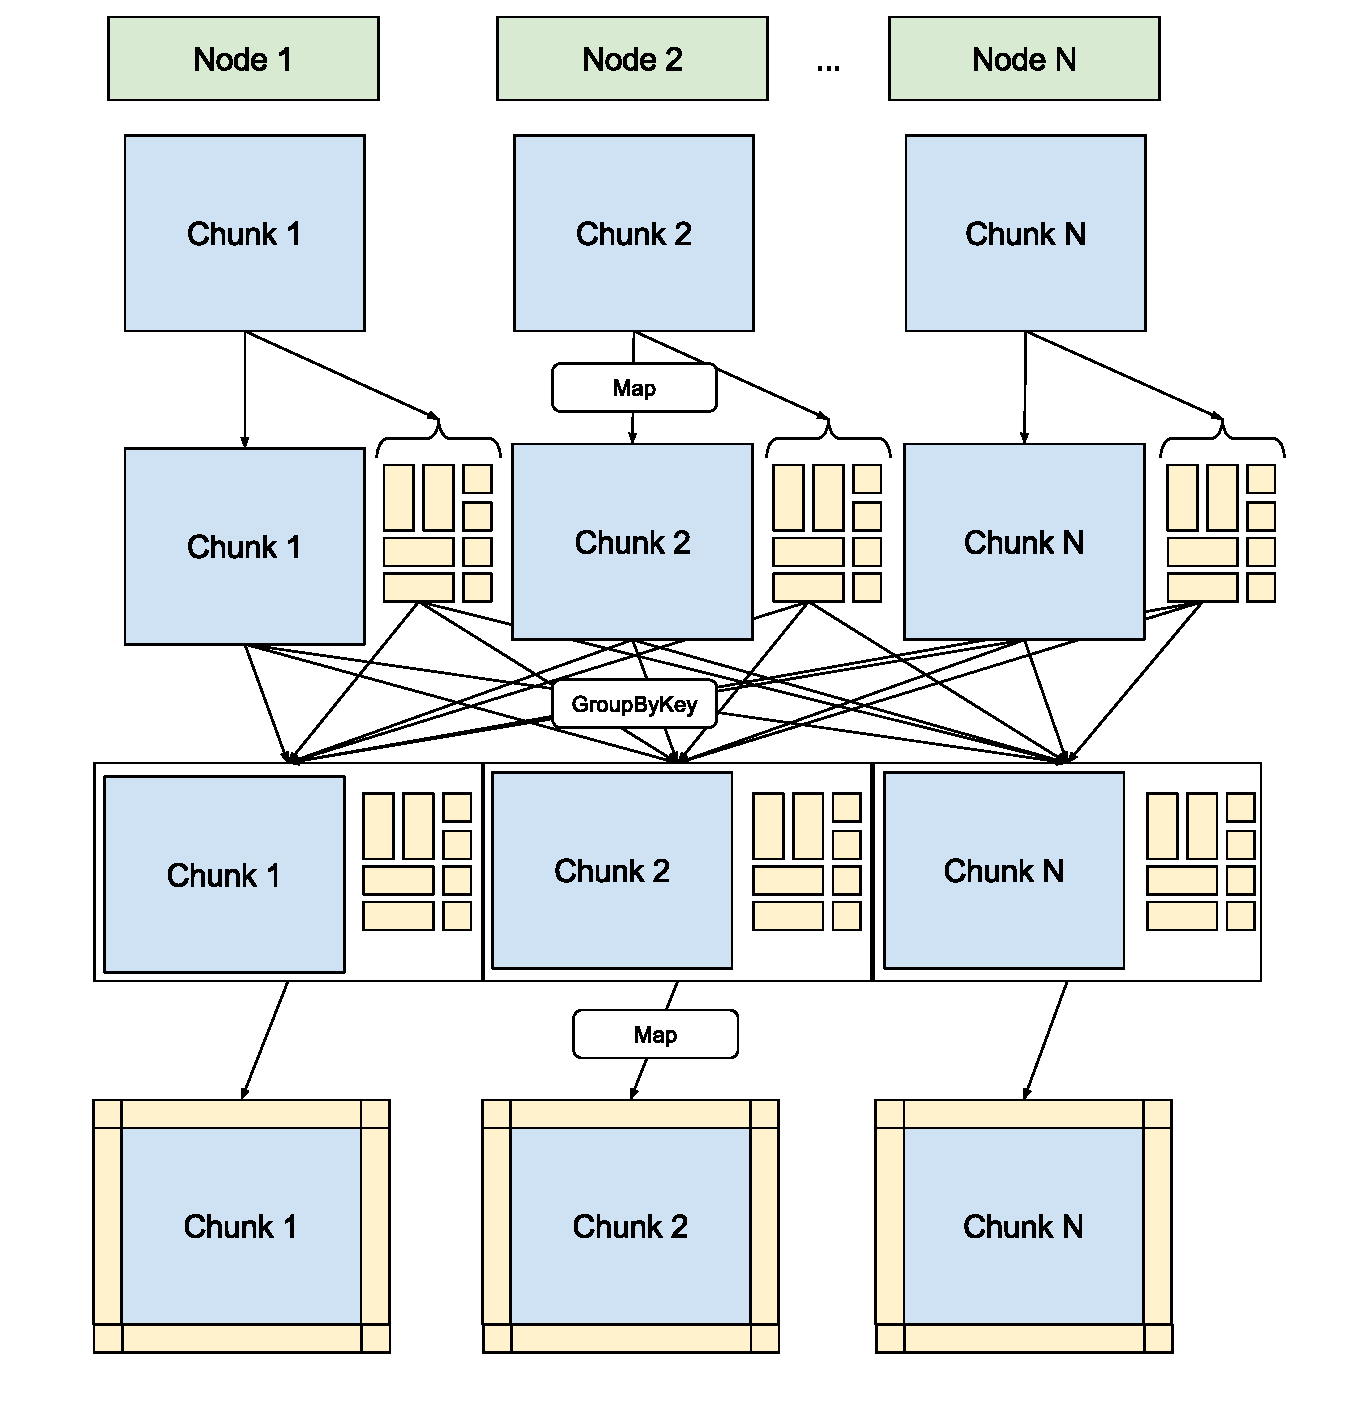
\includegraphics[width=0.9\textwidth]{images/MapGroup.eps}
\caption{Diagram of the the MapGroupByKey algorithm}
\label{fig:map_group}
\end{figure}

\section{MapCogroup}

Method described in this section was inspired by chapter 4 in \textit{Learning Spark}~\cite{learning_spark}.
It uses custom partitioner and two separate collections for chunks and neighbours
to prevent Spark from moving chunks around the network. It uses combination
of map and cogroup steps.

The first map operates on the same key-value pair collection as above. However,
now it transforms the collection into separate key-value pair collection of neighbours,
instead of creating one mixed one as was done previously (figure~\ref{fig:map_cogroup}).

In second step, the \texttt{cogroup} transformation is very similar to the grouping transformation
from the MapGroupByKey method, with the difference that in this case it operates on two collections 
instead of one. The result is the same as in previous sections.

In addition, the collection containing chunks is partitioned using custom partitioner.
The partitioner takes the key, which represents coordinates and outputs index of node
on which the chunk should be physically present. Using this partitioner spark
shuffles only the other collection, which contains neighbour data, over network and
keeps the chunks collection in place.

\begin{figure}
\centering
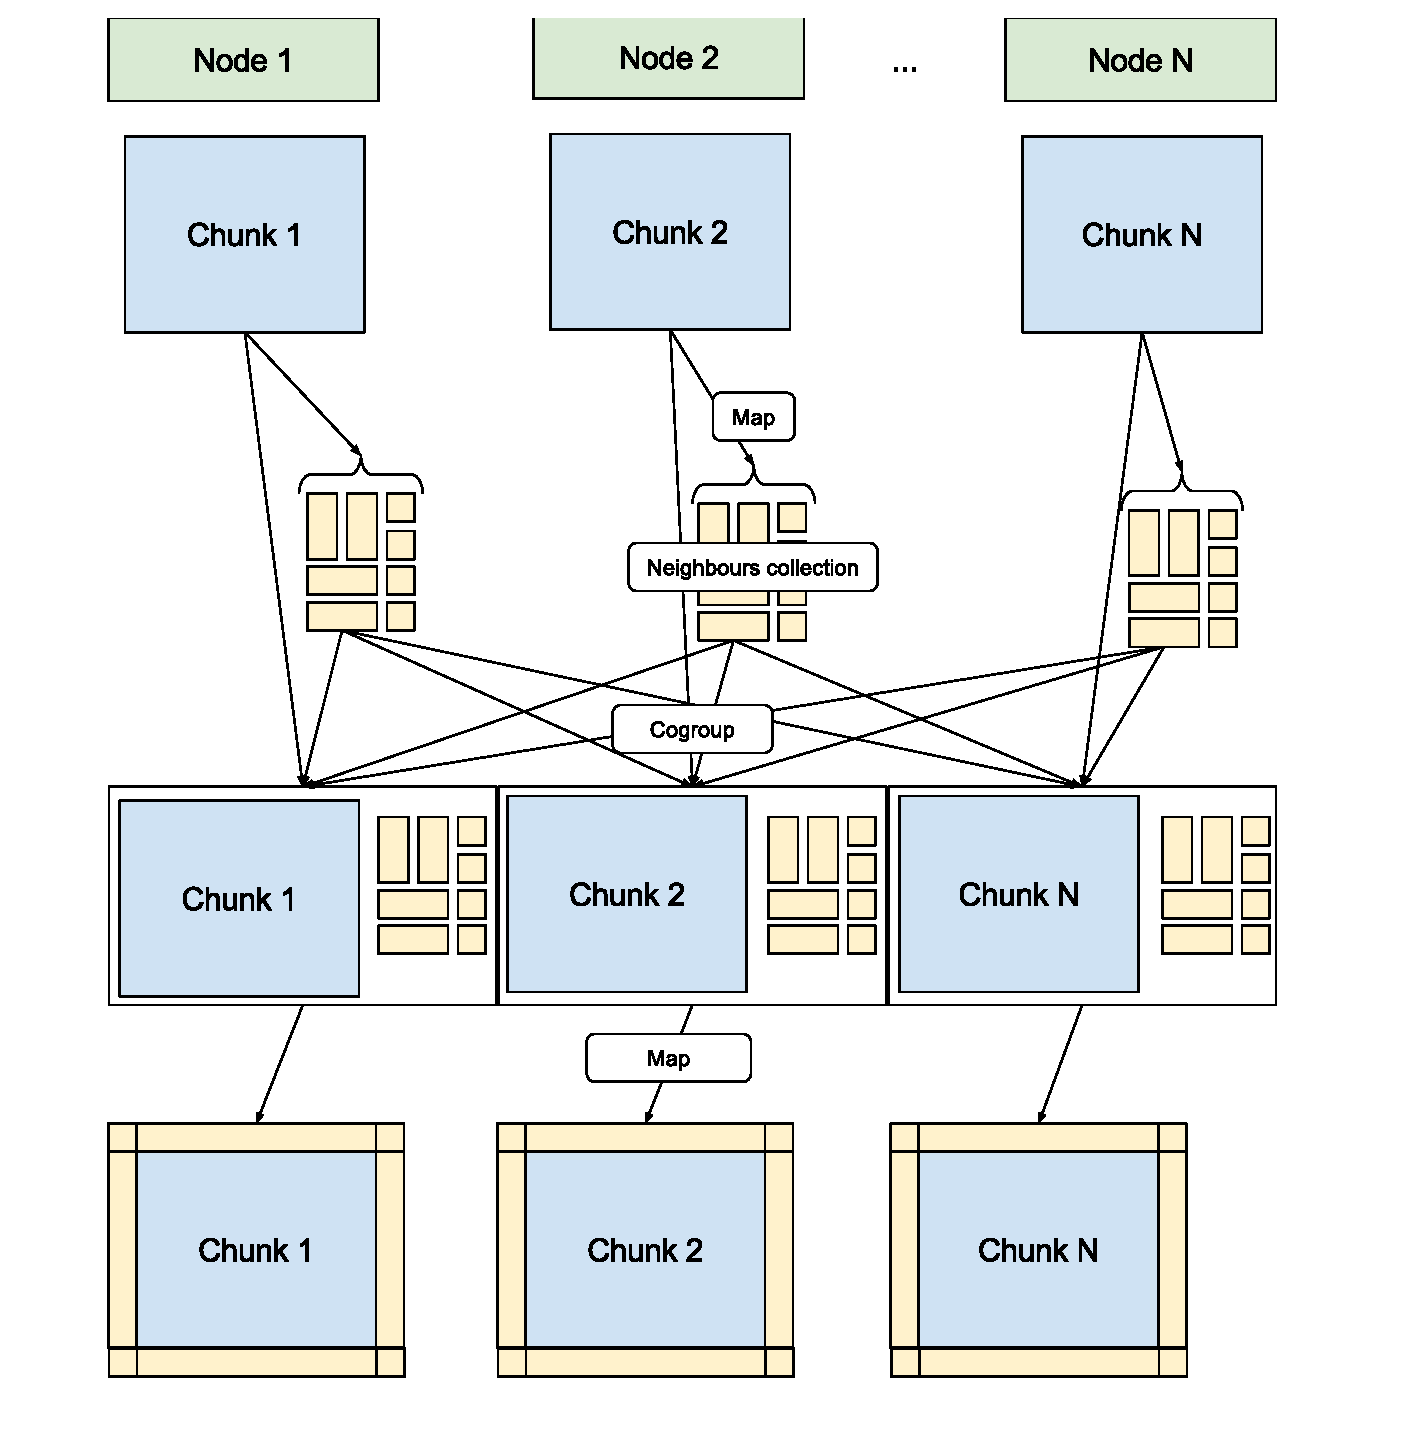
\includegraphics[width=0.9\textwidth]{images/MapCogroup.eps}
\caption{Diagram of the the MapCogroup algorithm}
\label{fig:map_cogroup}
\end{figure}

\section{Caching and checkpointing}

Spark uses lazy execution when running programs stages. This means that transformation
on a collection are saved in its lineage are executed only after a call
that materialises the collection on the driver program is called on it. Examples of such calls are
\texttt{count} that returns the number of items in the collection, \texttt{collect}
which returns array of all items in the collection or \texttt{reduce}, which, as opposed
to \texttt{reduceByKey} reduces the collection into single item. The lineage can
be imagined as a tree that contains child and parent relationships between tasks.

This introduces some issues. First issue is that often, when resolving stages that
do network shuffle, Spark executes the parent stages more than once. This is
considered standard Spark behaviour and is solved by caching the parent collection
using \texttt{cache} method, which also marks the collection to be explicitly reused
when executing child stages. However, it was found that Spark keeps more cached collections
than necessary, and therefore workaround was devised. Using this workaround, first,
new collection is created, then cached and materialised using \texttt{count} and 
then \texttt{unpersist} is called on the old collection to remove it from the cache.

Another issue is lineage length. In iterative algorithms, such as the ones described 
in this report, the lineage that Spark keeps in order to be able to restore execution
in the case of failure can get quite long. This results in significant slowdown of
Spark task resolution and eventually leads to stack overflow errors. One possible
solution is to increase JVM maximum stack memory, but the standard practice is to
\texttt{chekpoint} collections. This serialises the collection to disk and forgets
its lineage.

%==============================================================================
%  LES in Java
%==============================================================================
\chapter{LES in Java}
\label{chap:les_java}

This chapter deals with the second challenge, which is reimplementing LES in Java.
To do this, the OpenCL host code written in Fortran needs to be rewritten in
Java. The host code consists mainly of a \texttt{switch} construct, which executes
different routines in the OpenCL kernel in a loop. Next, methods for initialising variables,
constructing and deconstructing halos need to be created. Finally, the newly 
written Java OpenCL host code needs to be integrated with Spark.

\section{JNA with Fortran}

LES works with about 40 different variables that store states of different systems,
wind velocity, pressure, halos and grid constants. These variables need to be initialised
before the execution of the simulation and then passed to the kernel. This process is 
covered in a substantial part of the Fortran source code.

Since accessing the existing Fortran subroutines is a viable strategy
~\footnote{\url{http://www.javaforge.com/wiki/66061}},
it was decided to write a simple Fortran subroutine, which groups 
all subroutines that initialise the needed variables. The Fortran code
is then compiled into a shared library, and can be accessed from Java using
Java Native Access~\footnote{\url{https://github.com/java-native-access/jna}}.

\section{Aparapi for Unconventional Cores}

To write the OpenCL host code, Aparapi for Unconventional Cores (Aparapi-ucores)
~\cite{aparapi_ucores}
~\footnote{\url{https://gitlab.com/mora/aparapi-ucores}}
is used as an underlying library that facilitates communication
with the OpenCL kernel. It is a fork of Aparapi library that allows
running OpenCL code on unconventional cores such as FPGAs. In addition,
it allows running OpenCL kernels from precompiled binaries.

Aparapi allows to write Java code which is then translated into OpenCL kernel code
and executed. However, since LES kernel code is already written, this is 
unnecessary. It is impossible to disable this behaviour and therefore a 
workaround is necessary. Although, with binary flow, which is provided by Aparapi-ucores,
it is possible to execute compiled binary of the provided kernels instead of 
the kernels generated by Aparapi, Aparapi will still expect the same method signature as 
the one generated by Aparapi. Therefore it is needed to provide Aparapi with
dummy Java code, that translates into correct OpenCL method signature.
This can be achieved by using all parameters in correct order and the parameters
need to have correct datatype. Also, parameters that are supposed to be written to
by kernel need to be marked as such by assigning a value into them. Example dummy
code is in the listing below:

\begin{lstlisting}[language=Java]
  float[] p2;
  float[] uvw;
  float[] uvwsum;
  float[] fgh;

  @Override
  public void run() {
    float sum = p2[0] + uvw[0] + uvwsum[0] + fgh[0];
    uvw[0] = sum;
    uvwsum[0] = sum;
  }
\end{lstlisting}
The corresponding kernel method signature as generated by Aparapi:
\begin{lstlisting}[language=C]
__kernel void run(
   __global float *p2, 
   __global float *uvw, 
   __global float *uvwsum, 
   __global float *fgh,
   int passid
)
\end{lstlisting}
In the example above, four kernel parameters are used. All are arrays of floats.
Note that the order in which they are listed in the sum in the first line of the 
\texttt{run} method, is the same as the order of the parameters in the signature.
In addition the \texttt{uvw} and \texttt{uvwsum} variables were assigned into,
which marks them as kernel-writable inside Aparapi. Also important to note,
is final parameter \texttt{passid}, which is being automatically inserted by Aparapi,
and contains the id of the current kernel execution.

Due to this, there are some modification that need to be done to the OpenCL
kernel, before compiling into a binary. First, the \texttt{passid} needs to be added to
the parameter list. Second, Aparapi does not support passing non-constant scalar fields
into the kernel as parameter. As a workaround to this, scalar fields can be represented
as simple single item 1D arrays. Finally the name of the kernel method is restricted to
the name \texttt{run}. As of writing of this report, however, this was found not to be true
and it is possible to use different names, but the written code does not reflect this.

By default, Aparapi copies all parameters to and from kernel before and after every kernel
execution. This is due to large number of parameters in LES undesirable. Therefore, for
iterative applications, it is recommend to enable explicit Aparapi mode, which then requires
the programmer to call \texttt{put} and \texttt{get} methods to explicitly write and read 
parameters to and from the kernel.

\subsection{Device specific OpenCL binaries}

Since OpenCL is supposed to be compatible with wide range of devices, the same OpenCL
code can be executed on any OpenCL device. This is not true, however, for the 
compiled binaries, which are device specific. This means that new binaries need to 
be created whenever the simulation is to be run on a new device. There is no
tool available that allows easily compile kernel into binaries, but OpenCL specification
describes a method that allows to retrieve the compiled binary code
~\footnote{\url{https://www.khronos.org/registry/cl/sdk/1.0/docs/man/xhtml/clGetProgramInfo.html}}.
Therefore it was decide to create a simple compilation tool 
~\footnote{\url{https://github.com/adikus/cl-compile}}
which allows the user to specify a \texttt{.cl} kernel file and device with which to
compile the kernel file.

\subsection{Memory alignment}

Aparapi-ucores contains functionality which copies the contents of the parameters
into a memory aligned location. This is done because some devices such as FPGAs
do not interact well with unaligned memory locations and locations in JVM heap
might not be aligned. This functionality is currently experimental, and allocates 
new memory for every kernel-writable parameter every kernel execution. In addition to this,
it copies the content of parameters from the original JVM memory location to this new 
location and back every kernel execution for every parameter. This results in a significant 
slowdown in execution, which is undesirable.

This functionality can be turned off, since in theory, using unaligned parameters
should not pose any issues when running the kernel on CPUs and GPUs. However,
after switching this functionality off, it was found that the kernel no longer runs
properly on Intel CPUs. The reason remains, as of writing of this report, unknown.
Because of this, it was decided to modify the underlying Aparapi-ucores C++ source code
to create a workaround that deals with the excessive memory copies. The workaround
allocates the aligned memory location only once and copies the memory from or to it
only when the \texttt{get} or \texttt{put} Aparapi methods are called, and therefore
works only with the explicit Aparapi mode, which is used in this project.

\section{Halo construction and deconstruction}

Since LES has already been parallelised using MPI~\cite{les_mpi}, functionality 
for reading and writing halos is already implemented inside the OpenCL kernel code.
The format used by the implementation is a single 1D array for each halo and 
therefore needs to be deconstructed into eight different neighbours before sending and 
again constructed from neighbour arrays into single array again after receiving.

Since the spatial domain in this project is considered to be wrapped such that
bottom connects to top and left connects to right, this halo construction and 
deconstruction can be demonstrated and tested on a single node (figure~\ref{fig:halo_exchange}).

\begin{figure}
\centering
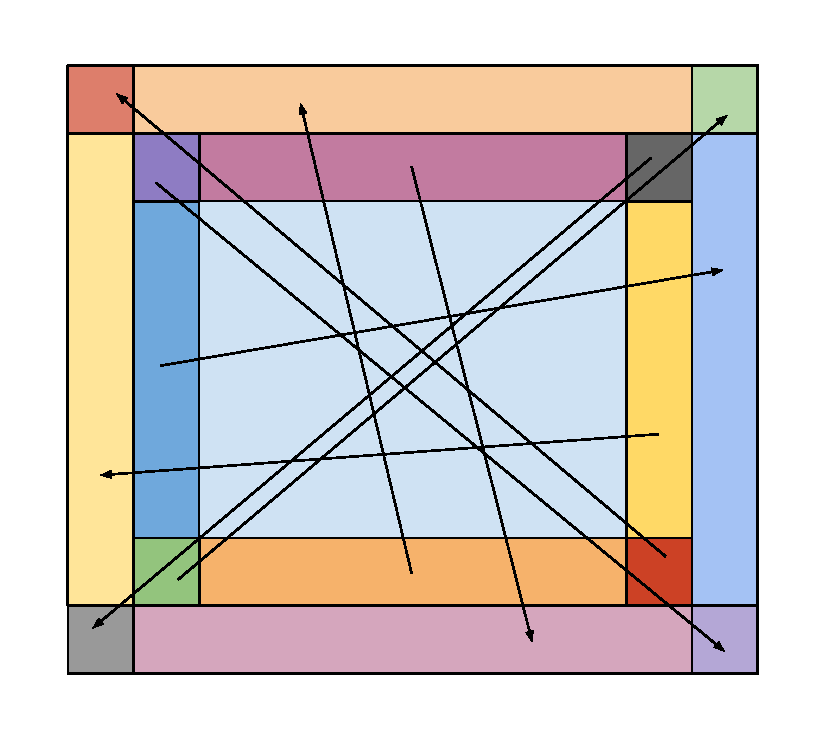
\includegraphics[width=0.5\textwidth]{images/Neighbour_exchange_2.eps}
\caption{Diagram of halo change on a single node}
\label{fig:halo_exchange}
\end{figure}

\section{LES in Apache Spark}

As a final part of the project implementation, working LES Aparapi implementation
needs to be integrated into Spark. MapCogroup approach described in \autoref{chap:halos}
is used as the halo exchange algorithm.

Each time step of the simulation is divided into 11 steps, with each step executing
OpenCL kernel once. The 8th step (\texttt{PRESS\_SOR}) is an exception. 
In this step the successive over relaxation is run, which requres multiple 
iterations of kernel executions. Normally the over relaxation is run until 
the simulation state converges, but in this project it was decided to use constant
number of 50 iterations.

Each kernel execution needs to be accompanied be a halo write beforehand 
and halo read afterwards, both of which are an extra kernel execution.
After each group of halo write, simulation step and halo read the appropriate halos
should be exchanged over network. In addition some simulation steps do a reduction over 
the whole domain, which means that a reduction over the nodes needs to be done using Spark.

Table~\ref{tab:les_stages} contains the summary of each stage.

\begin{center}
  \begin{tabular}{ | l | l | l | }
      \hline
      \# & Stage & Halo exchange, reduction \\
      \hline
      1 & \texttt{VELNW\_\_BONDV1\_INIT\_UVW} & \texttt{p}, \texttt{uvw} and \texttt{uvwum} halo exchange \\
      2 & \texttt{BONDV1\_CALC\_UOUT} & \texttt{uvw} halo exchange \\
      3 & \texttt{BONDV1\_CALC\_UVW} & \texttt{uvw} halo exchange \\
      4 & \texttt{VELFG\_\_FEEDBF\_\_LES\_CALC\_SM} & \texttt{uvw}, \texttt{uvwsum}, \texttt{fgh}, 
      \texttt{diu} and \texttt{sm} halo exchange \\
      5 & \texttt{LES\_BOUND\_SM} & \texttt{sm} halo exchange \\
      6 & \texttt{LES\_CALC\_VISC\_\_ADAM} & \texttt{fgh} and \texttt{fgh\_old} halo exchange \\
      7 & \texttt{PRESS\_RHSAV} & \texttt{rhs} and \texttt{fgh} halo exchange + reduction \\
      8 & \texttt{PRESS\_SOR} & 
      \begin{tabular}[t]{@{}l@{}}
        \texttt{p} halo exchange, there are three kernel executions for each SOR \\
         iteration, which means three halo exchanges per iteration \\
        + one reduction per iteration to determine the convergence value 
      \end{tabular} \\
      9 & \texttt{PRESS\_PAV} & \texttt{p} halo exchange + reduction \\
      10 & \texttt{PRESS\_ADJ} & \texttt{p} halo exchange \\
      11 & \texttt{PRESS\_BOUNDP} & \texttt{p} halo exchange \\
      \hline
  \end{tabular}
  \captionof{table}{Summary of halo exchanges and reductions for each LES stage in one time step}
  \label{tab:les_stages}
\end{center}

Spark collection that holds the kernel hosts on each node consists of key value pairs.
The key is represented by an integer which has value between 0 and X*Y-1, where X and Y
are the size of the node grid. For example, if X is 2 and Y is 3, it means we intend to
run the simulation on cluster with 6 worker nodes and each node is running a simulation
on a 150x150x90 size domain. The value in the key value pair is represented by a subclass
of Aparapi Kernel class.

The neighbours are represent by a Neighbour class which encapsulates the underlying data
array and the direction from which it came (N,S,W,E,NW,NE,SW,SE).

Finally, helper methods have been created for executing steps of simulation, exchanging halos
and reductions. This means that a execution of a single simulation step can be written similarly to:

\begin{lstlisting}
// 7th stage - PRESS_RHSAV
kernels = executeKernelStep(kernels, States.PRESS_RHSAV);
kernels = HaloExchanger.exchangeHalos(kernels, "rhs,fgh", ip, jp, kp, X, Y);
kernels = divisionReduction(kernels);
\end{lstlisting}

\subsection{Lineage \& Checkpointing}
\label{chap:lineage_n_checkpointing}

The fact that single timestep of the simulation needs to be represented by
large number of jobs (10 stages * 2 [execution + halo exchange] + 50 SOR iterations * 3
* 2 = 320; this is just an approximation) means that lineage grows very quickly.
With the recommended rate of chekpointing, which is once per 100 jobs, three 
checkpoints are created every time step of the simulation. Since one time step
should not take longer than couple of seconds, this means that large quantity 
of data is serialised to disk over the run of program.

This can create problems when trying to execute the simulation in environment
with restricted disk space. Therefore another workaround was devised, which deletes
all previous checkpoints before creating a new one. Checkpoints in Spark are used
to recover from a crash of a node or a similar scenario. However in our case,
recovering is not as simple as deserialising a class from disk. Further work
would have to be done to initialise the OpenCL kernel and load the recovered  
parameters into it. This was deemed to be out of the scope of this project.
Therefore the checkpoints are completely useless and can be deleted without worry.

%==============================================================================
%  Evaluation
%==============================================================================
\chapter{Evaluation}
\label{chap:eval}

Evaluation in this chapter was done to determine, whether the approach to parallelisation
developed in this project is a competitive alternative to MPI.

Small number of tests was run without Spark to determine the true runtime of
the simulation without overheard caused by Spark.

The final tests were done on a network cluster, with number of nodes varying from one
to eight. However only very small number of tests was conducted, due to 
project timing issues (too close to deadline). Under normal circumstances,
tests with higher number of nodes and different number of time steps would be run.
In addition, all tests would be run multiple times.

\section{Architecture}

All tests were done on GPG cluster of CS department at University of Glasgow
~\footnote{\url{http://www.dcs.gla.ac.uk/research/gpg/cluster.htm}}.
The cluster consists of 20 nodes, each having 64GB of RAM and 2 Intel Xeon processors
~\footnote{\url{http://ark.intel.com/products/75267/Intel-Xeon-Processor-E5-2640-v2-20M-Cache-2_00-GHz}}.
Three nodes of the cluster are available to public and therefore only the rest 17 are
suitable for running experiments.

\section{Baseline tests}

Two baseline tests were done. First runs LES as it would be run without any
parallelisation over network. Second does the same, but adds halo writes and reads
as well as simple halo exchanges as show in figure~\ref{fig:halo_exchange}.
Another test was done using Spark local mode. In this mode both the driver 
program and Spark worker run in a single JVM container. Each test was run twice and 
all tests were run using 100 time steps. The results were measured using the \texttt{time} command
and can be seen in table~\ref{tab:baseline_times}. Commands used to run these tests can be seen below:
\begin{verbatim}
  path-to-project/LES$ bash scripts/single.sh 100
  path-to-project/LES$ bash scripts/halos.sh 100
  path-to-project/LES$ bash scripts/spark_cpu_standalone.sh 100 1 1
\end{verbatim}

\begin{center}
  \begin{tabular}{ | l | r | r | }
      \hline
      Test & \#1 (s) & \#2 (s) \\
      \hline
      Single LES & 41.216 & 40.146 \\
      LES with simple halos & 73.313 & 74.676 \\
      Spark local & 1337.929 & 1354.030 \\
      \hline
  \end{tabular}
  \captionof{table}{Execution times of baseline tests}
  \label{tab:baseline_times}
\end{center}

\section{Spark tests - increasing domain size}

The final tests done using spark were done on varying number of nodes with expanding domain.
The aim is to increase the total domain size by increasing the number of nodes.
Each node runs computation on a domain of size 150x150x90, which means that the simulation
on 8 nodes with configuration 2x4 will have total domain size 300x600x90. Spark master
and the driver program were run on a cluster node separate from the other nodes.
Each test was run only once and with 100 time steps. The results are measured using the \texttt{time} command
and can be seen in figure~\ref{fig:eval}. Commands used to run these tests can be seen below
(see appendix~\ref{chap:running} to find out how to run Spark master and workers):
\begin{verbatim}
  path-to-project/LES$ bash scripts/spark-submit.sh 100 X Y
\end{verbatim}
where X and Y are the sizes of the node grid.

\begin{figure}
\centering
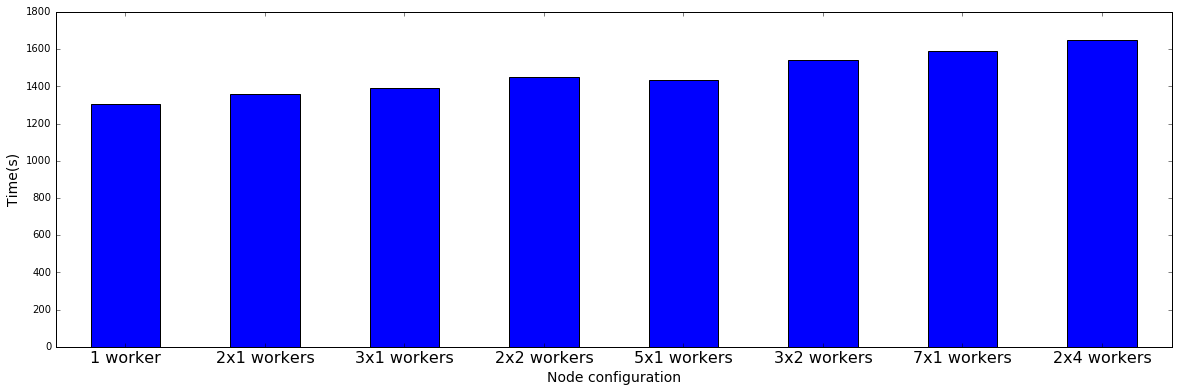
\includegraphics[width=1\textwidth]{images/evaluation.png}
\caption{Bar chart with runtimes of the 100 time steps of simulation for various node configurations}
\label{fig:eval}
\end{figure}

\section{Discussion}

The tests report about 20x slowdown of the simulation run time with Spark compared to
the baseline tests. Ratio of overhead caused by spark to time spent in the simulation
seems to be too high. In addition, a linear increase in run time with increasing number of nodes
can be observed. This means that as is, the approach taken in this project might not
be suitable to parallelising LES. However, due to very small number of tests, 
this is not a conclusive result. The next chapter goes into detail as to what tests
should be done next, in order to make a proper conclusion.

%==============================================================================
%  Conclusion
%==============================================================================
\chapter{Conclusion}
\label{chap:conclusion}

\section{Future Work}

While this project has proven that it is indeed possible to parallelise LES
on a network cluster using Apache Spark, the first evaluation results are
not favourable. However there is still some testing and evaluation to be done
to determine whether using this approach to parallelisation of LES is usable.

\subsection{Spark overhead}

The biggest issue that is causing the adverse performance seems to be overhead
caused by Spark. While single kernel execution together with one halo write and
one halo read takes only tens of milliseconds, the time it takes Spark
to run the task and exchange the halos seems to be much higher. Spark reports
that time spent executing tasks is less than half of the overall execution time, which means
that most time is spent scheduling tasks and resolving lineage.

One possible explanation of the high overhead might be the need to recompute the
lineage after each network shuffle. Since Spark cannot predict where each item
in the collection will end up after the shuffle, it might need to recompute the 
lineage after every shuffle. The fact that shuffle is necessary
in each halo exchange, and that these are done more than 100 time per steps could
potentially mean high frequency of Spark recalculating the lineage.

One approach to decrease the overhead could be to try different versions of Spark.
Evaluation in this project was done using version 1.4.1, however since Spark 
seems to be rapidly moving project, there are already newer versions (1.5, 1.6), 
which could have improved performance.

Another approach is to increase kernel execution time. This could be done by increasing
domain size per node. This would be decrease the ratio of Spark overhead time to 
execution time, which would decrease the overall slowdown from 15-20x to 
something more manageable. The cluster on which the evaluation was done, has 64GB
of memory per node available and during the evaluation just above tenth of that
has been used, so increasing the domain is a viable strategy.

\subsection{Checkpointing}

Another factor resulting in the poor performance is the frequent checkpointing
(mentioned in \autoref{chap:lineage_n_checkpointing}). The fact the the program
is writing checkpoints to disk means that a lot of time is spent waiting until
it is finished. One possible solution is to write to a faster medium. In the evaluation
the checkpoint directory was on a Network File System, which means that even 
writing to standard HDD might improve the performance. Other options are using SSD
or even mounted ramfs. The best approach, however, would be to disable checkpointing
entirely. While this is not possible in Spark currently, it is possible to rewrite 
the source code, since Spark is an open source project.

\subsection{Evaluation on massively parallel cluster}

The largest test during evaluation done in this project was done on eight nodes.
While the results show almost linear increase in computational time with
increasing number of nodes, it cannot be assumed that this trend continues.
Therefore it is important to test the simulation on cluster with tens, hundreds,
or potentially even thousands nodes. If the computation proves to scale well
on such large clusters, the current slowdown would be offset by the 
possibility of running the simulation on much larger domain than what is
currently possible.

\subsection{Broadcast variables}
The approach proposed in \autoref{chap:broadcast} was initially dismissed due to 
unnecessary network transfers. However, since it was found that the bottleneck 
is caused by Spark overhead and not the network transfers, this approach
might prove to be surprisingly effective. This approach consists essentially only 
of two map steps, and thus no network shuffle is needed, which should make Spark
evaluate the lineage much more efficiently. However, since this approach needs
to transfer all the neighbour data to the driver program, this approach might
not be usable when running the simulation on a massively parallel cluster (e.g. 1000s of nodes).

\section{Summary}

The aim of this project was to explore whether it is possible to parallelise 
LES using Apache Spark. The produced result proves that it is possible, but only 
with a large performance trade off. While it allows to run the simulation on larger
domain and provides a way to nicely abstract the halo exchanges, at the current stage
it does not provide suitable alternative to MPI. However, further work is needed
to determine, whether the limitations discovered in this project can be overcome.

%%%%%%%%%%%%%%%%
%              %
%  APPENDICES  %
%              %
%%%%%%%%%%%%%%%%
\begin{appendices}

\chapter{Running the simulation}
\label{chap:running}

The project files that are required to run the parallelised version of LES can be found on GitHub.
~\footnote{\url{https://github.com/adikus/hurricaneProject}}
The repository contains modified version of Aparapi-ucores (in \texttt{/aparapi-ucores}), 
the Game of Life proof of concept (in \texttt{/dummy}),
and the parallelised simulation code in \texttt{/LES}.

\section{Building Aparapi-ucores (\texttt{/aparapi-ucores})}

\begin{itemize}
\item Install OpenCL drivers for your system. (AMD APP SDK
~\footnote{\url{http://developer.amd.com/tools-and-sdks/opencl-zone/amd-accelerated-parallel-processing-app-sdk/}} 
used in project)
\item Make sure environmental variable \texttt{LD\_LIBRARY\_PATH} contains path to OpenCL libraries
\item Build Aparapi using \texttt{ant build} in \texttt{src/aparapi}. Configuration in \\
\texttt{src/aparapi/com.amd.aparapi.jni/build.xml} might be neeeded
\end{itemize}

\section{Running Game of life proof of concept (\texttt{/dummy})}

\begin{itemize}
\item Download Apache Spark~\footnote{\url{http://spark.apache.org/}} (project tested with version 1.4.1)
\item Build project using \texttt{mvn package}
\item To run the cogroup version:
\begin{verbatim}
path/to/spark/bin/spark-submit \
  --class hoos.project.dummy.DummyPartitionedJoin \
  --master local[8] \
  target/dummy-map-reduce-0.1.jar data/gol.txt data/out.txt N
\end{verbatim}
where first two arguments are the input and ouptut files and N is the number of iterations.
\texttt{local[8]} means it will run on 8 CPU threads
\end{itemize}

\section{Running LES (\texttt{/LES})}

\begin{itemize}
\item Build Aparapi-ucores (above)
\item Download Apache Spark
\item Configure \texttt{scripts/conf.cfg}
\begin{verbatim}
APARAPI_PATH=/path/to/project/aparapi-ucores/src/aparapi
SPARK_PATH=/path/to/spark/
IP=192.168.1.64 # IP address of Spark master
WORK_DIR=/temp/or/scratch
MGRID_FILE_PATH=/path/to/project/GIS/Tokyo_20mgrid.txt

APARAPI_JNI_PATH=$APARAPI_PATH/com.amd.aparapi.jni/dist
APARAPI_JAR_PATH=$APARAPI_PATH/com.amd.aparapi/dist/aparapi.jar
\end{verbatim}

\item Build project using \texttt{mvn package}

\item To run version without Spark you can run either of:
\begin{verbatim}
  path-to-project/LES$ bash scripts/single.sh N
  path-to-project/LES$ bash scripts/halos.sh N
\end{verbatim}
where halos also runs single node halo exchanges and N is the number of iterations.

\item For local mode Spark versions, run either of:
\begin{verbatim}
  path-to-project/LES$ bash scripts/spark_cpu_standalone.sh N X Y
  path-to-project/LES$ bash scripts/spark_gpu_standalone.sh N X Y
\end{verbatim}
to run wither on CPU or GPU and X and Y are sizes of the node grid. 
Note: if you specify more than 1x1 node grid, these will run sequentially.

\item To run on cluster:
  \begin{itemize}
  \item Start Spark master
  \begin{verbatim}
  export SPARK_MASTER_IP=192.168.1.64
  sh path/to/spark/sbin/start-master.sh
  \end{verbatim}
  where 192.168.1.64 is replaced with the IP address configured in \texttt{conf.cfg}
  \item Start one or more workers (run on the target node)
  \begin{verbatim}
  path-to-project/LES$ bash scripts/start_cpu_worker.sh
  path-to-project/LES$ bash scripts/start_gpu_worker.sh
  \end{verbatim}
  \item Submit spark application
  \begin{verbatim}
  path-to-project/LES$ bash scripts/spark-submit N X Y
  \end{verbatim}
  \item You can monitor the cluster in Spark WebUI at \url{http://localhost:8080/}
  \end{itemize}

\end{itemize}

\section{Creating shared library from Fortran code}

The Fortran source code is not available on GitHub but in SVN repository at School of CS at University of Glasgow.

\begin{itemize}
\item Configure and install \url{https://github.com/wimvanderbauwhede/OpenCLIntegration}
\item Run \texttt{scons -f SConstruct.ocl\_lib} in \texttt{RefactoredSources}
\item \texttt{libles\_ocl.so} should have been created
\end{itemize}

\end{appendices}

%%%%%%%%%%%%%%%%%%%%
%   BIBLIOGRAPHY   %
%%%%%%%%%%%%%%%%%%%%

\bibliographystyle{plain}
\bibliography{bib}  

%%%%%%%%%%%%%%%%%%%
%   ???????????   %
%%%%%%%%%%%%%%%%%%%
%\begin{verbatim}
%H. Nakayama, T. Takemi, H. Nagai, and E. Agency,
%“Coupling of WRF and building-resolving urban CFD
%models for analysis of strong winds over an urban
%area,” 3rd International Workshop on Nonhydrostatic
%Numerical Models, vol. 3, no. RIKEN AICS, Kobe,
%Japan, 2014.
%\end{verbatim}

\end{document}
